% 12 variables in here:
% H_1 = 10.0, H_2 = 10.0, H_3 = 10.0, U_1 = 0.0, U_2 = 0.0, U_3 = 0.0, h_1 = 10.0, h_2 = 10.0, h_3 = 10.0, u_1 = 0.0, u_2 = 0.0, u_3 = 0.0
\begin{figure}[h!]
  \centering
  % \subfigure[] {
  % 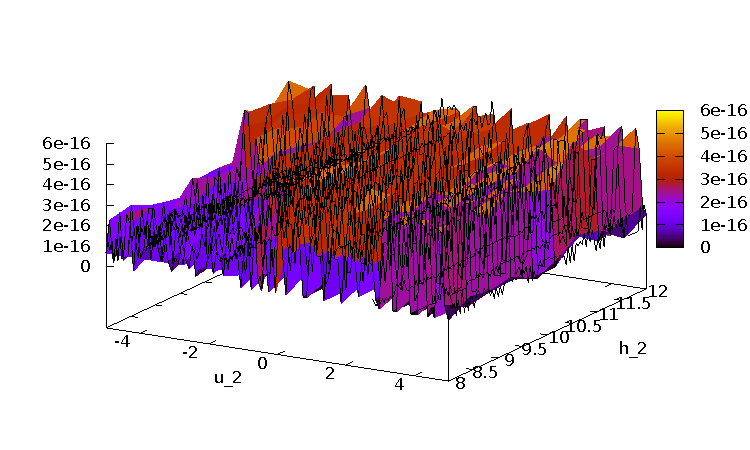
\includegraphics[scale=\zoomfactor]{{{equidist_2_default/10.0_10.0_0.0_0.0_10.0_y_0.0_xf00}}}
  % }
  \subfigure[] {
    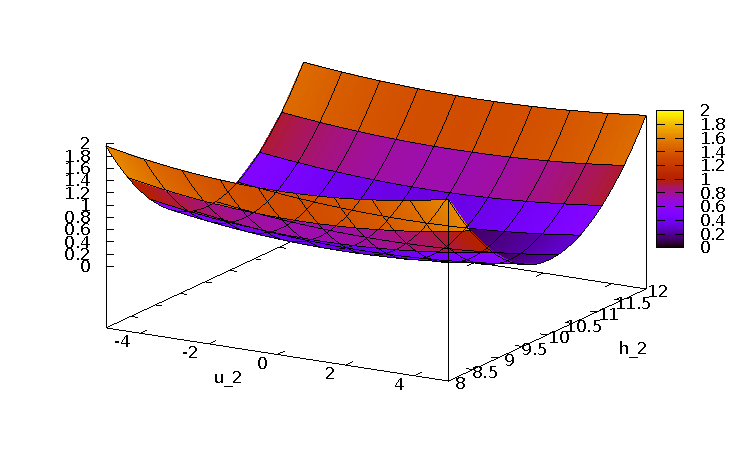
\includegraphics[scale=\zoomfactor]{{{equidist_2_default/10.0_10.0_0.0_0.0_10.0_y_0.0_xf01}}}
  }
  % \subfigure[] {
  % 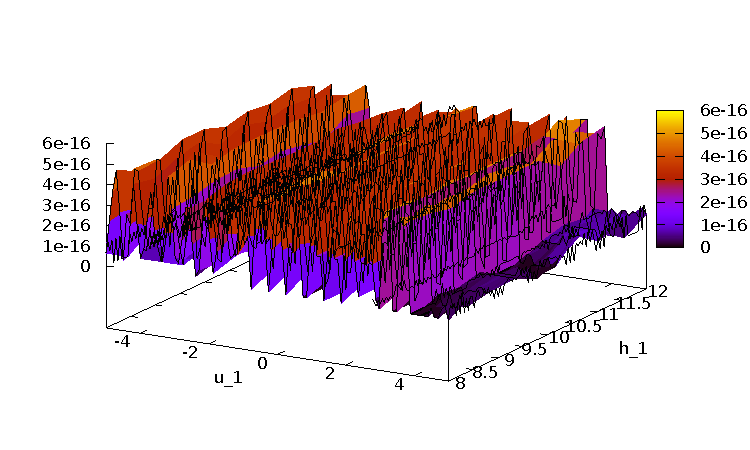
\includegraphics[scale=\zoomfactor]{{{equidist_2_default/10.0_10.0_0.0_0.0_y_10.0_x_0.0f00}}}
  % }
  \subfigure[] {
    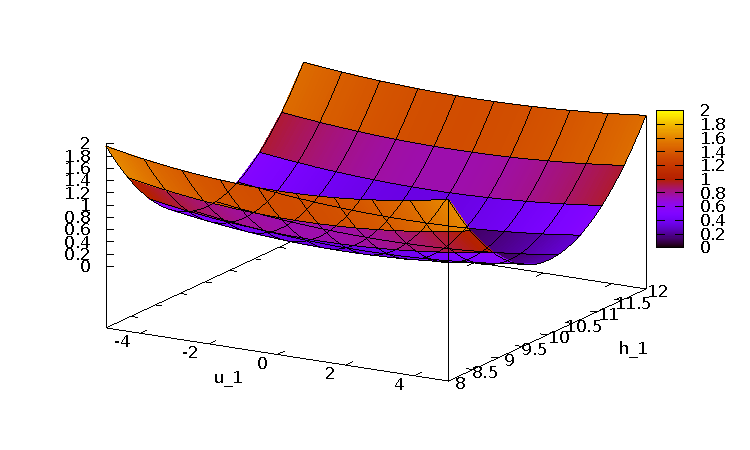
\includegraphics[scale=\zoomfactor]{{{equidist_2_default/10.0_10.0_0.0_0.0_y_10.0_x_0.0f01}}}
  }

  \subfigure[]{
    \begin{tikzpicture}
      \node at (0,0) {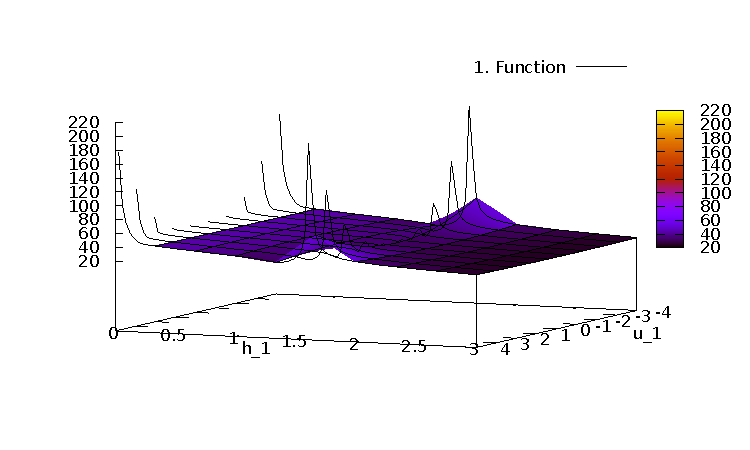
\includegraphics[scale=\zoomfactor]{{{2_punkte_alles_10_0/x_y_0.0_10.0_0.0_10.0_0.0_10.0f1}}}};
      \fill[white] (.8,1.2) rectangle (1.75,1.5);
      \node[align=right, text width=3cm] at (.2,1.33) {\textsf{\tiny{Impulse error}}};
    \end{tikzpicture}
  }
  \subfigure[]{
    \begin{tikzpicture}
      \node at (0,0) {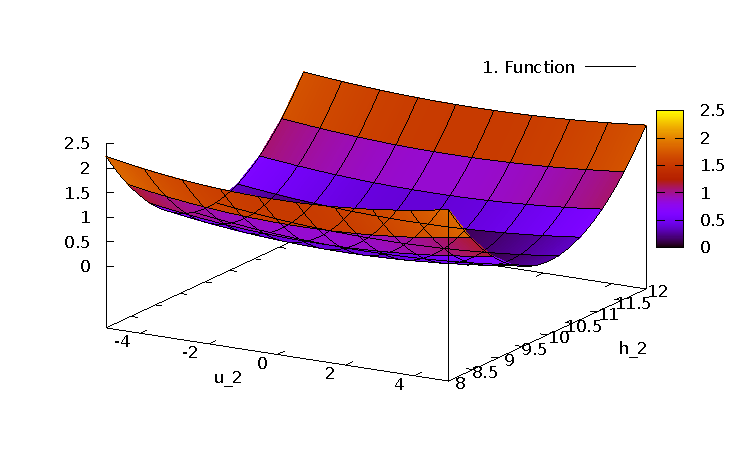
\includegraphics[scale=\zoomfactor]{{{2_punkte_alles_10_0/0.0_10.0_0.0_10.0_x_y_0.0_10.0f1}}}};
      \fill[white] (.8,1.2) rectangle (1.75,1.5);
      \node[align=right, text width=3cm] at (.2,1.33) {\textsf{\tiny{Impulse error}}};
    \end{tikzpicture}
  }

  \caption{}
  \label{fig:equidist_2_default}
\end{figure}

%%% Local Variables:
%%% TeX-master: "../results.tex"
%%% End:
